\documentclass[12pt,letterpaper]{article}
\usepackage[utf8]{inputenc}
\usepackage{times}
\usepackage{authblk}
\usepackage{graphicx}
\usepackage{placeins}
\usepackage{pdfpages}

\title{StudyUp - Design an Implementation of your System (DIS)}

\author[1]{Yukon Vinecki}
\author[2]{Chandler Petersen}
\author[3]{Calvin Todorovich}
\author[4]{Moyez Ikhlas}
\affil[1]{vineckiy, EECS - Oregon State University}
\affil[2]{petercha, EECS - Oregon State University}
\affil[3]{todorovc, EECS - Oregon State University}
\affil[4]{ikhlasm, EECS - Oregon State University}

\usepackage[parfill]{parskip}
\begin{document}

\pagenumbering{roman}
\maketitle
\clearpage
\tableofcontents
\clearpage
\pagenumbering{arabic}

\section{UML Class Diagrams}
\begin{figure}[!htb]
  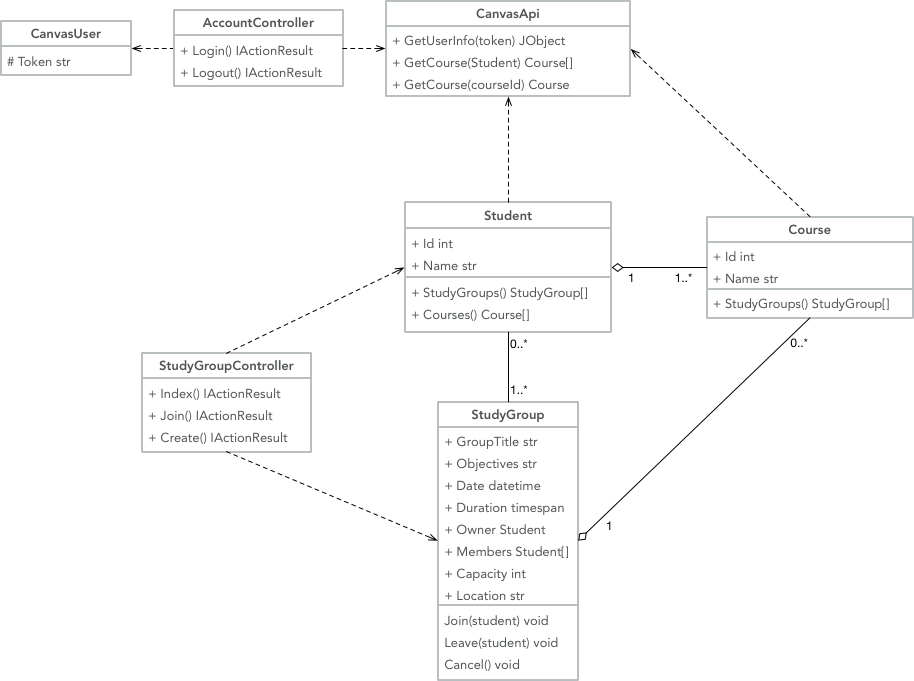
\includegraphics[width=\linewidth]{StudyUp_Class_Diagram.png}
  \caption{Class Diagram}
  \label{class_diagram}
\end{figure}
\clearpage
\section{Packages}
Our implementation utilizes MVC (Model, View, Controller) allowing for a separation of concern for different parts of our program. Each area is cohesive containing the information it is responsible for. The Model deals with the data that is used in the application. The View contains the html and styling for the website the user views. The Controller handles processing requests and completing actions. Another advantage of using MVC is it reduces coupling as each controller is completely independent from each other. Allowing specific components to be modified without affecting the functionality of others. 

For our project there are four primary packages, Models, Views, Controllers, and Canvas. The first three contain what was discussed previously while Canvas contains code relating to interfacing with Canvas using their REST api. This was done as Canvas is an outside resource and as such should be isolated from our core codebase.

\section{Design Patterns}
\textbf{Observer}

The Observer design pattern would be useful for implementing the "View Study Group" portion of the application. It would wait for output data to be generated by the user, and once that happens, other users will be notified of the change. In this way, users can see when other users create or update new or existing study groups, then view and respond to the relevant information. An event handler triggered by these changes would alert the viewing users, or simply update the data so they could see it. 

\textbf{Builder}

We will likely use the Builder pattern for user authentication. For user authentication for the application, we will be utilizing the Canvas API so users can login using their canvas credentials, as well as use their current course information to create and join study groups. Handling multiple users and secure authentication requires a layer of complexity that would be difficult to develop. Using the Canvas API encapsulates the related complicated objects necessary to handle these operations. In doing so, we can add on new blocks to build off of the code without changing the authentication code we already have. 
% I think this is a relevant choice for this pattern ... 
% Perfect choice, this is the exact pattern used for converting the JSON response into a usable object.

We will also use the Builder pattern for creating each study group record that will later be placed in the back-end database. The builder would be able to create these records easily, and it would not matter where we put them after. 

\textbf{Decorator}

We will use the Decorator design pattern for modifying the functionality of the "View Study Group" module. This module changes depending on what type of user you are. If you are a group administrator, it gives you the option to edit the group details, and then to "create" or "cancel" the group. However, if you are user looking at an existing group, you have the option to either "join" or "leave" the group. Of course, this type of user cannot edit the form, as they did not create the group. Since the Decorator pattern helps modify the characteristic or functionality of the object at runtime, it would be an ideal pattern for this situation. This pattern will keep us from having to make redundant objects for each type of user.

\textbf{Strategy}

The Strategy design pattern will be used for the StudyUp homepage. The homepage differs in appearance depending on the state of the user's data. If the user have already joined several study groups, their homepage will display all of their active groups and a summary of the important information pertaining to each of those groups. However, in the case that the user has not joined any study groups, the Create Study Group UI will be the default homepage. The strategy pattern is the ideal choice as it allows for selection of an algorithm at runtime, and addresses behavioral patterns. Essentially, the homepage will need to execute entirely different modules on runtime depending on the state of the user's information. The strategy pattern will be especially adept at handling this sort of changing behavioral behavior. 

\clearpage
\section{Exceptions and Handling} % If you think of any more, feel free to add them! Also, I think this is what they want. All the exceptions used are from the .NET documentation. 
\textbf{Exception:} User attempts to enter invalid string into form. This will throw an InvalidArgumentException. 

\textbf{Exception Handler:} Alerts user that their entry is invalid, and gives example of proper format. In addition, for fields with a finite amount of options, such as time, there will be a drop-down menu where the user can select a valid time, which avoids the exception scenario entirely. 

\textbf{Exception:} User attempts to create or join a study group that conflicts with one they have already joined or created. This will be handled by a InvalidOperationException. This exception is thrown when the state of the object cannot support a particular method being attempted for the object instance.

\textbf{Exception Handler:} Notify user that the study group they are trying to join has a time conflict with an existing study group that they either created, or have joined. This alert will notify that they need to either cancel the previous study group (either their membership or the group entirely, if they are the administrator), or that they cannot create/join the new group during that time-span. In this way, conflict will be avoided.

\textbf{Exception:} The study group administrator attempts to cancel a study group that already has more than 3 members who have joined. This will throw a GroupNotEmptyException. % Exception is the base object, SEHException is thrown when code outside the C# runtime throws an exception. -Yukon

\textbf{Exception Handler:} This exception will be handled by offering the remaining members in the group the option to take over administrator privileges for that study group. If one of the users accepts this, they are now the group administrator and have control to edit the group details. The prior group administrator can then remove themselves from the group without deleting the already established study group. 

\clearpage
\section{Meeting Report}
Chandler, Calvin, and Yukon were able to meet on Tuesday to work on the UI. The past week each group member worked on their portion of the UI, following the prototypes worked out in the last meeting. Yukon finished the user authentication portion for the application, Chandler finished the View Study Group UI, and Calvin is nearing completion with the create UI.

Our goals for next week are for each member to begin implementing the functionality for their portion of the UI/application. Chandler will work on the View functionality, Yukon will continue work on canvas integration, Calvin will work on implementing the Create Study Group functionality, and Moyez will work on the Find Study Group functionality. By next week, our goal is to have a rough functional version of the website.

We plan to meet sometime during the week to review progress we have made, discuss any changes or issues, and continue working on the implementation.
\end{document}